\documentclass{article}
\usepackage[utf8x]{inputenc}
\usepackage[frenchb]{babel}
\usepackage[T1]{fontenc}
\usepackage{lmodern}
\usepackage{fullpage}
\usepackage{graphicx}
\usepackage{epstopdf}
\usepackage{caption}
\usepackage{subcaption}
\usepackage{multirow}

% Math symbols
\usepackage{amsmath}
\usepackage{amssymb}
\usepackage{amsthm}
% Numbers and units
\usepackage[squaren, Gray]{SIunits}
\usepackage{sistyle}
%\usepackage[autolanguage]{numprint}
%\usepackage{numprint}
\newcommand\si[2]{\numprint[#2]{#1}}
\newcommand\np[1]{\numprint{#1}}

\DeclareMathOperator{\pgcd}{pgcd} % use \dif instead

\DeclareMathOperator{\newdiff}{d} % use \dif instead
\newcommand{\dif}{\newdiff\!}
\newcommand{\fpart}[2]{\frac{\partial #1}{\partial #2}}
\newcommand{\ffpart}[2]{\frac{\partial^2 #1}{\partial #2^2}}
\newcommand{\fdpart}[3]{\frac{\partial^2 #1}{\partial #2\partial #3}}
\newcommand{\fdif}[2]{\frac{\dif #1}{\dif #2}}
\newcommand{\ffdif}[2]{\frac{\dif^2 #1}{\dif #2^2}}
\newcommand{\constant}{\ensuremath{\mathrm{cst}}}
\newcommand{\bigoh}{\ensuremath{\mathcal{O}}}

% cfr http://en.wikibooks.org/wiki/LaTeX/Colors
\usepackage{color}
\usepackage[usenames,dvipsnames,svgnames,table]{xcolor}
\definecolor{dkgreen}{rgb}{0.25,0.7,0.35}
\definecolor{dkred}{rgb}{0.7,0,0}

\usepackage{listings}
\lstset{
  numbers=left,
  numberstyle=\tiny\color{gray},
  basicstyle=\rm\small\ttfamily,
  keywordstyle=\bfseries\color{dkred},
  frame=single,
  commentstyle=\color{gray}=small,
  stringstyle=\color{dkgreen},
  %backgroundcolor=\color{gray!10},
  %tabsize=2,
  rulecolor=\color{black!30},
  %title=\lstname,
  breaklines=true,
  framextopmargin=2pt,
  framexbottommargin=2pt,
  extendedchars=true,
  inputencoding=utf8x
}
\lstset{language={matlab}}

\title{Devoir 4}
\author{Arnaud Cerckel \and Benoît Legat \and
Nicolas Stevens \and Harold Taeter}

\newcommand{\Ha}{\mathcal{H}}

\begin{document}

\maketitle

\section{Question 1}
\subsection{Équations du mouvement}
Soit le système hamiltonien à deux corps, d'invariant $\Ha (p,q)$ où $p$ est la vitesse de chaque corps et $q$ leur position \footnote{On a évidemment $p(t)$ et $q(t)$. Pour une planète, la composante $p_1$ représente sa vitesse dans la direction "$x$" du plan et la composante $p_2$, sa vitesse dans la direction "$y$" du plan.}. Considérons tout d'abord un système où un des deux corps a une masse beaucoup considérablement plus élevé que l'autre, ce qui le rend statique. On a alors 
$$\Ha (p,q) = \frac{1}{2} p^T p - \frac{1}{||q||_2} . $$
On sait que $\dot{\Ha}(p,q) = 0$ car $\Ha$ est invariant dans le temps.
De plus, comme (par la règle de dérivée en chaîne)
\[
  \dot{\Ha}(p,q) = \fpart{\Ha(p,q)}{p}^T\dot{p} + \fpart{\Ha(p,q)}{q}^T\dot{q},
\]
on doit avoir
\[
  \fpart{\Ha(p,q)}{q}^T\dot{q} + \fpart{\Ha(p,q)}{p}^T\dot{p} = 0.
\]

Les équations
\begin{align*}
  \dot{q} & = \fpart{\Ha(p,q)}{p} & \dot{p} & = -\fpart{\Ha(p,q)}{q}
\end{align*}
donnent
\begin{align*}
  \fpart{\Ha(p,q)}{q}^T\dot{q} + \fpart{\Ha(p,q)}{p}^T\dot{p} & =
  \fpart{\Ha(p,q)}{q}^T\fpart{\Ha(p,q)}{p} - \fpart{\Ha(p,q)}{p}^T\fpart{\Ha(p,q)}{q}\\
  & = 0
\end{align*}
ce qui respecte bien l'invariance temporelle de $\Ha$.

Soient $f_1(q,p)$ et $f_2(q,p)$ tels que
\begin{align*}
  \dot{q} & = f_1(q,p)\\
  \dot{p} & = f_2(q,p),
\end{align*}
on calcule
\begin{align*}
  f_1(q,p) & =  \fpart{\Ha (p,q)}{p}\\
  & =
  \begin{pmatrix}
    \fpart{}{p_1} \left(\frac{1}{2}(p_1^2 + p_2^2) - \frac{1}{\sqrt{q_1^2 + q_2^2}}\right)\\
    \fpart{}{p_2} \left(\frac{1}{2}(p_1^2 + p_2^2) - \frac{1}{\sqrt{q_1^2 + q_2^2}}\right)
  \end{pmatrix}\\
  & =
  \begin{pmatrix}
    p_1\\
    p_2
  \end{pmatrix}\\
  & = p\\
%
  f_2(q,p) & =  -\fpart{\Ha (p,q)}{q}\\
  & =
  -\begin{pmatrix}
    \fpart{}{q_1} \left(\frac{1}{2}(p_1^2 + p_2^2) - \frac{1}{\sqrt{q_1^2 + q_2^2}}\right)\\
    \fpart{}{q_2} \left(\frac{1}{2}(p_1^2 + p_2^2) - \frac{1}{\sqrt{q_1^2 + q_2^2}}\right)
  \end{pmatrix}\\
  & =
  \frac{-1}{2(q_1^2 + q_2^2)^{3/2}}
  \begin{pmatrix}
    2q_1\\
    2q_2
  \end{pmatrix}\\
  & = \frac{-q}{\|q\|_2^3}.
\end{align*}
Les équations du mouvement sont donc données par : 
$$\left\lbrace
\begin{array}{ccc}
\dot{q} &=& p\\
\dot{p} &=&  \frac{-q}{\|q\|_2^3}
\end{array}
\right.$$

\subsection{Description des méthodes numériques}
Nous souhaitons intégrer ces systèmes d'équations différentiels non-linéaires (de forme générale $y'(t) = f(t,y)$, où $y$ désigne aussi bien un scalaire qu'un vecteur) par des méthodes numériques : 
\begin{itemize}
\item la méthode d'Euler explicite, $y_{n+1} = y_n + h f(t,y_n)$
\item la méthode d'Euler implicite, $y_{n+1} = y_n + h f(t,y_{n+1})$ qui demande de résoudre une équation non-linéaire de type $g(y_{n+1})=0$, qu'on résoudra en utilisant la méthode itérative de Newton-Raphson
\item la méthode d'Euler symplectique qui est une combinaison des méthodes d'Euler implicite et explicite (on applique le schéma implicite à une composante de $y$ et un schéma explicite à l'autre). 
\end{itemize}

On remarque que $f_1(q,p) = f_1(p)$ et $f_2(q,p) = f_2(q)$.
On va utiliser cette propriété qui va nous être particulièrement utile pour Euler symplectique.
Pour Euler implicite, on aura besoin de
\begin{align*}
  \fpart{f_1(p)}{p} & = I\\
  \fpart{f_2(q)}{q} & =
  \begin{pmatrix}
    \fpart{}{q_1}\frac{-q_1}{(q_1^2 + q_2^2)^{3/2}} &
    \fpart{}{q_2}\frac{-q_1}{(q_1^2 + q_2^2)^{3/2}}\\
    \fpart{}{q_1}\frac{-q_2}{(q_1^2 + q_2^2)^{3/2}} &
    \fpart{}{q_2}\frac{-q_2}{(q_1^2 + q_2^2)^{3/2}}
  \end{pmatrix}\\
  & =
  -\begin{pmatrix}
    \frac{(q_1^2 + q_2^2)^{3/2} + 3q_1^2(q_1^2 + q_2^2)^{1/2}}{(q_1^2 + q_2^2)^3} &
    \frac{3q_1q_2}{(q_1^2 + q_2^2)^{5/2}}\\
    \frac{3q_1q_2}{(q_1^2 + q_2^2)^{5/2}} &
    \frac{(q_1^2 + q_2^2)^{3/2} + 3q_2^2(q_1^2 + q_2^2)^{1/2}}{(q_1^2 + q_2^2)^3}
  \end{pmatrix}\\
  & =
  -\begin{pmatrix}
    \frac{4q_1^2 + q_2^2}{(q_1^2 + q_2^2)^{5/2}} &
    \frac{3q_1q_2}{(q_1^2 + q_2^2)^{5/2}}\\
    \frac{3q_1q_2}{(q_1^2 + q_2^2)^{5/2}} &
    \frac{q_1^2 + 4q_2^2}{(q_1^2 + q_2^2)^{5/2}}
  \end{pmatrix}\\
  & =
  \frac{-1}{\|q\|_2^{5/2}}
  \begin{pmatrix}
    4q_1^2 + q_2^2 &
    3q_1q_2\\
    3q_1q_2 &
    q_1^2 + 4q_2^2
  \end{pmatrix}
\end{align*}

L'équation que Newton-Raphson devra résoudre à chaque pas est la suivante
\begin{align*}
  q_{k+1} & = q_k + hf_1(p_{k+1})\\
  p_{k+1} & = p_k + hf_2(q_{k+1})
\end{align*}
ou encore
\begin{align*}
  q_k - q_{k+1} + hf_1(p_{k+1}) & = 0\\
  p_k + hf_2(q_{k+1}) - p_{k+1} & = 0
\end{align*}
On doit donc résoudre $g(u) = 0$ où
$u =
\begin{pmatrix}
  q_{k+1}\\
  p_{k+1}
\end{pmatrix}$
et
\[
  g
  \left(
    \begin{pmatrix}
      q_{k+1}\\
      p_{k+1}
    \end{pmatrix}
  \right) =
  \begin{pmatrix}
    q_k - q_{k+1} + hf_1(p_{k+1})\\
    p_k + hf_2(q_{k+1}) - p_{k+1}
  \end{pmatrix}
\]
d'où
\[
  \fpart{g}{u}
  \left(
    \begin{pmatrix}
      q_{k+1}\\
      p_{k+1}
    \end{pmatrix}
  \right) =
  \begin{pmatrix}
    -I & h\fpart{f_1}{p}(p_{k+1})\\
    h\fpart{f_2}{q}(q_{k+1}) & -I
  \end{pmatrix}.
\]
Appliquons a présent ces méthodes sur un cas concret où la planète mobile a comme caractéristiques initiales : $p_0 = \begin{matrix}
0\\
2
\end{matrix}
$ et $q_0 = \begin{matrix}
0.4\\
0
\end{matrix} 
$.\\

\subsection{Comparaison des méthodes numériques}
Nous allons appliquer à ce cas les différentes méthodes d'intégration numérique pour 100 000 pas de temps dont la valeur est $h=5e-4$ (Euler implicite et explicite) ou $h=5e-2$ (Euler symplectique). Les résultats sont donnés à la figure \ref{fig:q1}


\begin{figure}
  \centering
  \begin{subfigure}[b]{0.3\textwidth}
    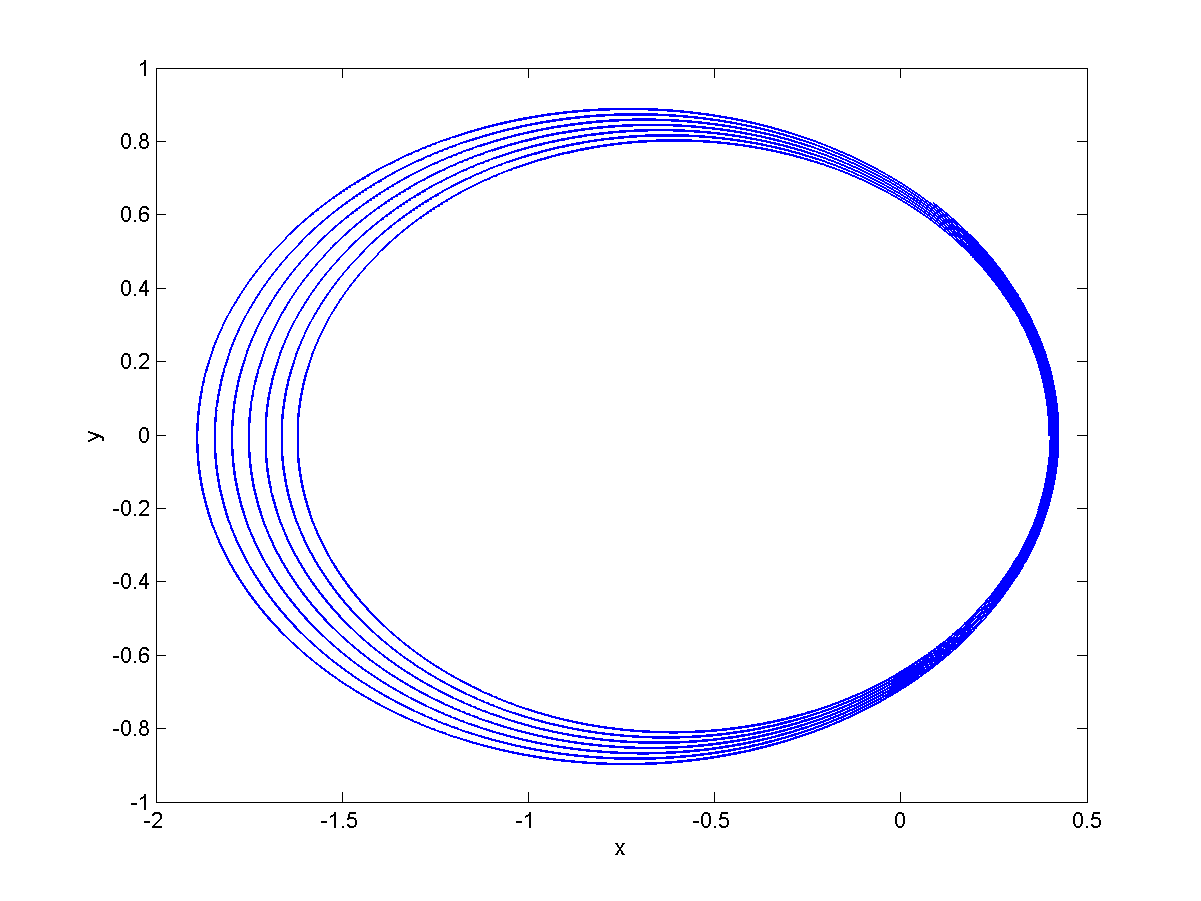
\includegraphics[width=\textwidth]{images/Q1_explicite_q.png}
    \caption{$q$ pour explicite}
    \label{fig:q1_explicite_q}
  \end{subfigure}%
  ~ %add desired spacing between images, e. g. ~, \quad, \qquad etc.
  %(or a blank line to force the subfigure onto a new line)
  \begin{subfigure}[b]{0.3\textwidth}
    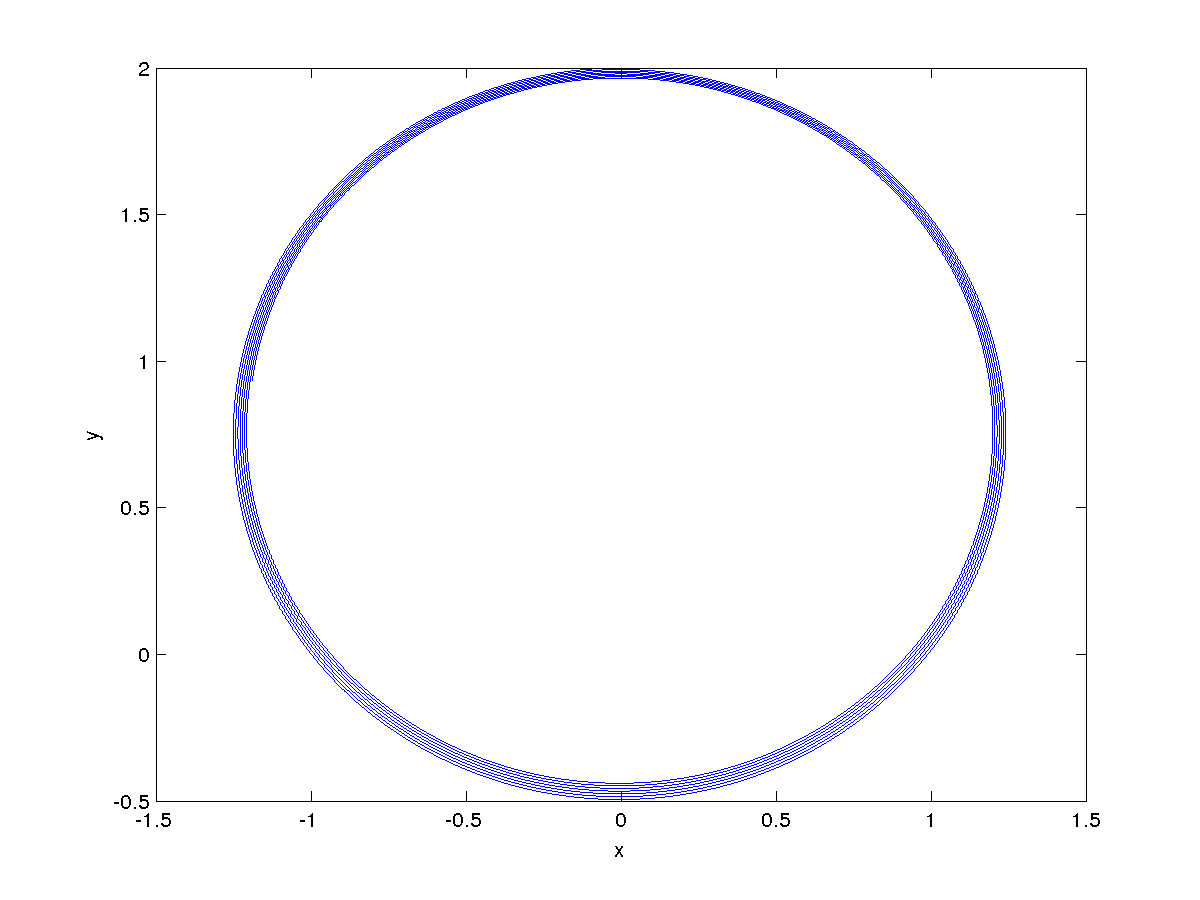
\includegraphics[width=\textwidth]{images/Q1_explicite_p.png}
    \caption{$p$ pour explicite}
    \label{fig:q1_explicite_p}
  \end{subfigure}
  ~
  \begin{subfigure}[b]{0.3\textwidth}
    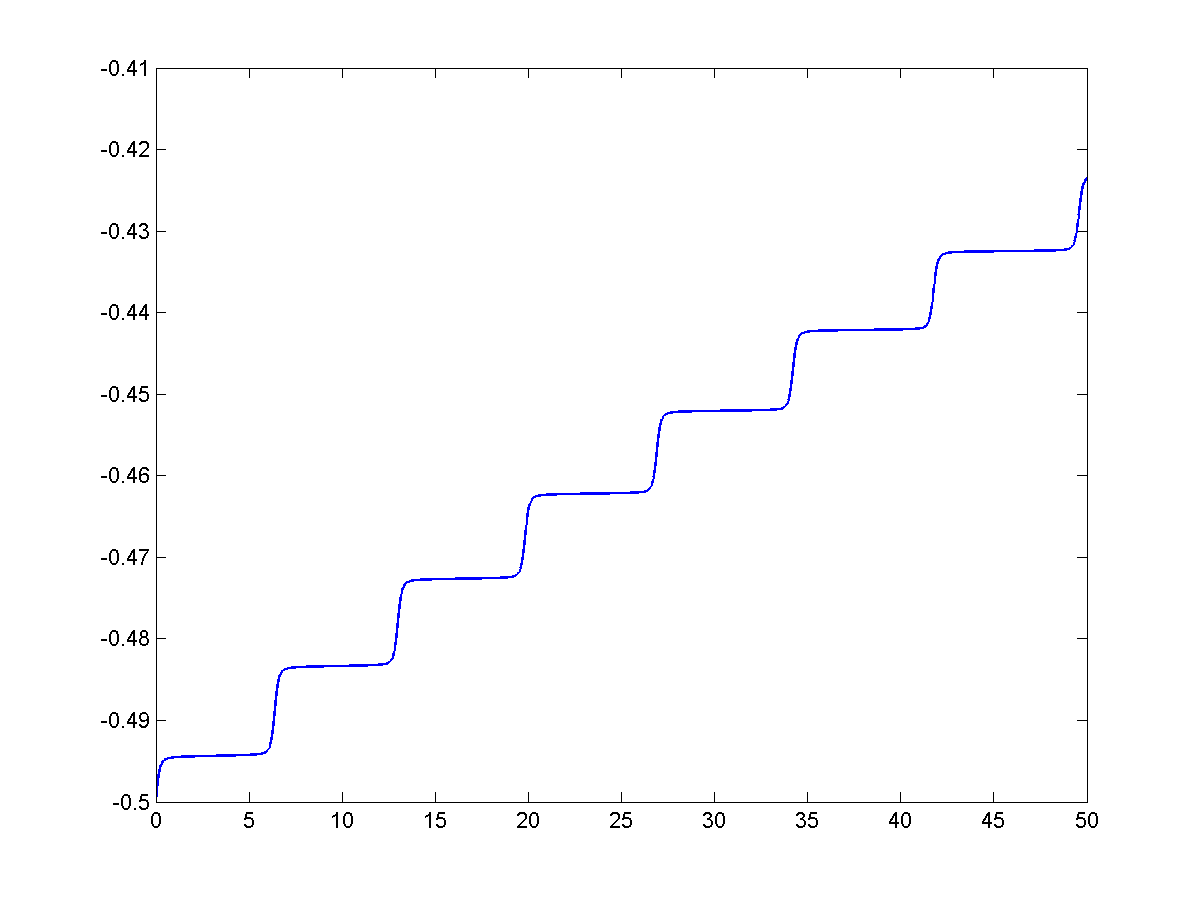
\includegraphics[width=\textwidth]{images/Q1_explicite_H.png}
    \caption{$\Ha$ pour explicite}
    \label{fig:q1_explicite_H}
  \end{subfigure}
  \begin{subfigure}[b]{0.3\textwidth}
    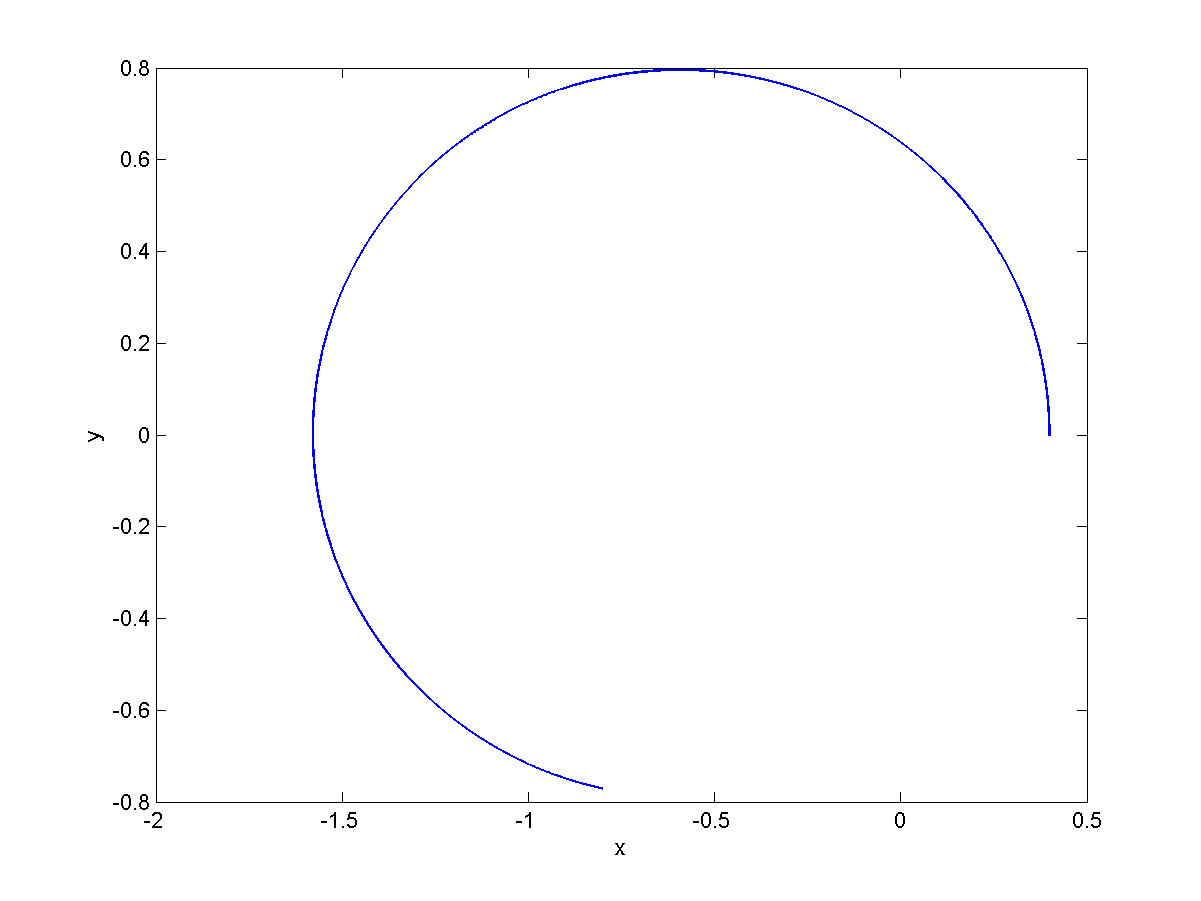
\includegraphics[width=\textwidth]{images/Q1_implicite_q.png}
    \caption{$q$ pour implicite}
    \label{fig:q1_implicite_q}
  \end{subfigure}%
  ~
  %(or a blank line to force the subfigure onto a new line)
  \begin{subfigure}[b]{0.3\textwidth}
    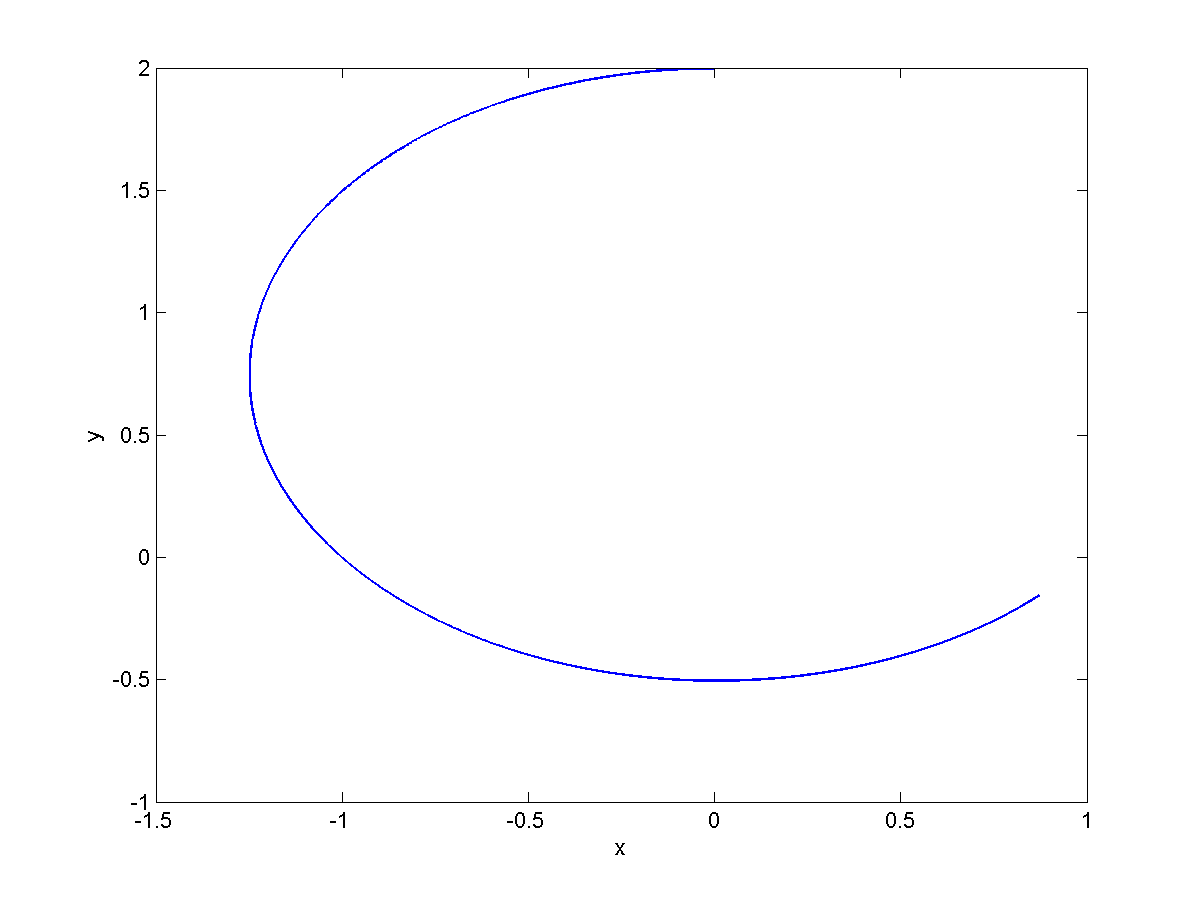
\includegraphics[width=\textwidth]{images/Q1_implicite_p.png}
    \caption{$p$ pour implicite}
    \label{fig:q1_implicite_p}
  \end{subfigure}
  ~
  \begin{subfigure}[b]{0.3\textwidth}
    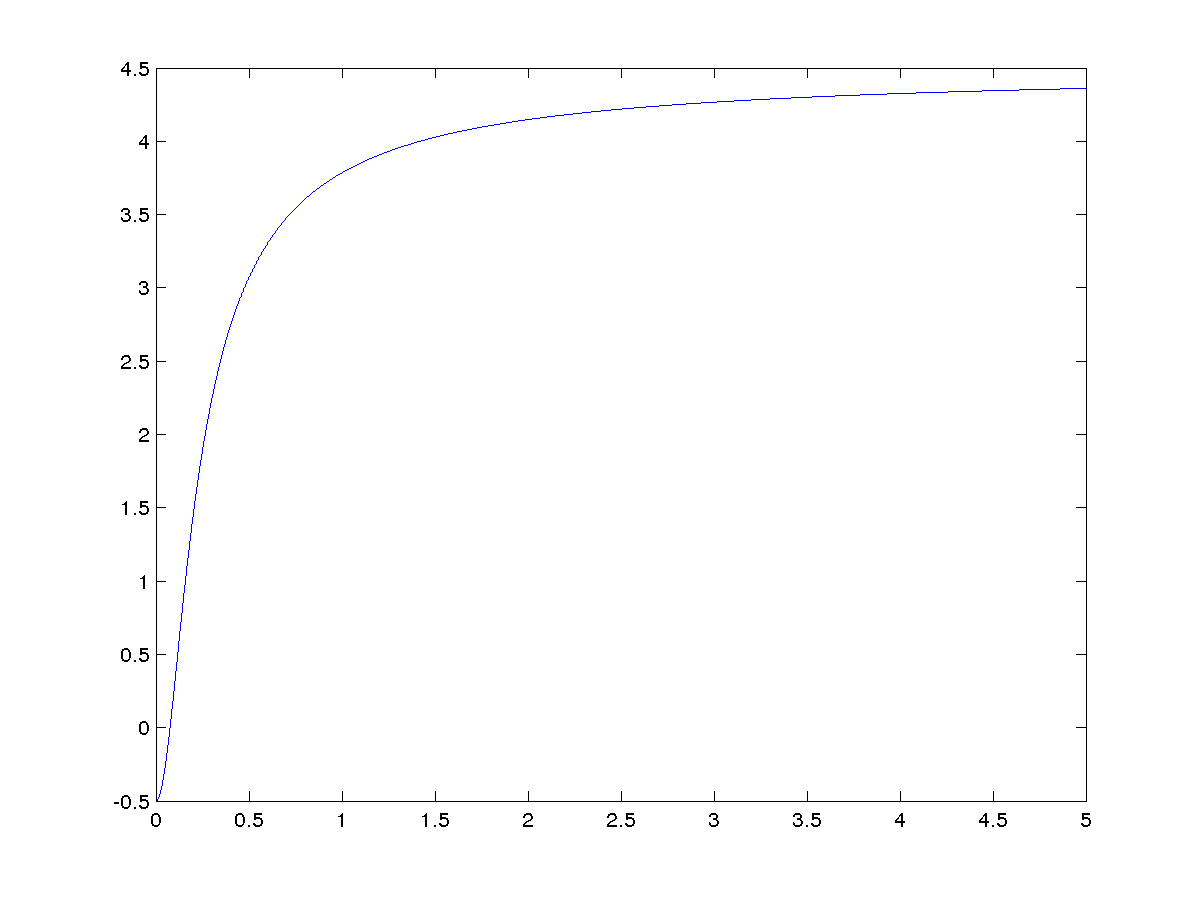
\includegraphics[width=\textwidth]{images/Q1_implicite_H.png}
    \caption{$\Ha$ pour implicite}
    \label{fig:q1_implicite_H}
  \end{subfigure}

  \begin{subfigure}[b]{0.3\textwidth}
    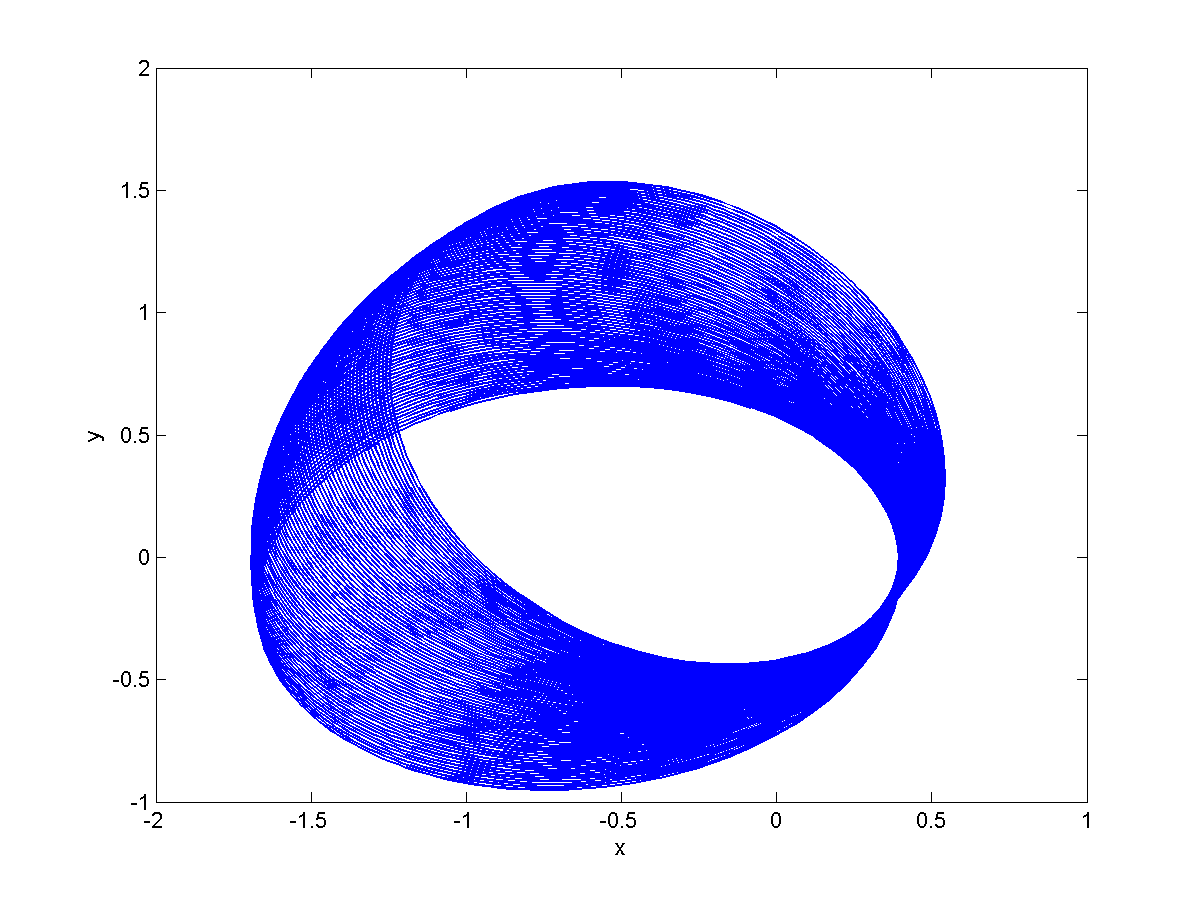
\includegraphics[width=\textwidth]{images/Q1_symplectique1_q.png}
    \caption{$q$ pour symplectique1}
    \label{fig:q1_symplectique1_q}
  \end{subfigure}%
  ~
  %(or a blank line to force the subfigure onto a new line)
  \begin{subfigure}[b]{0.3\textwidth}
    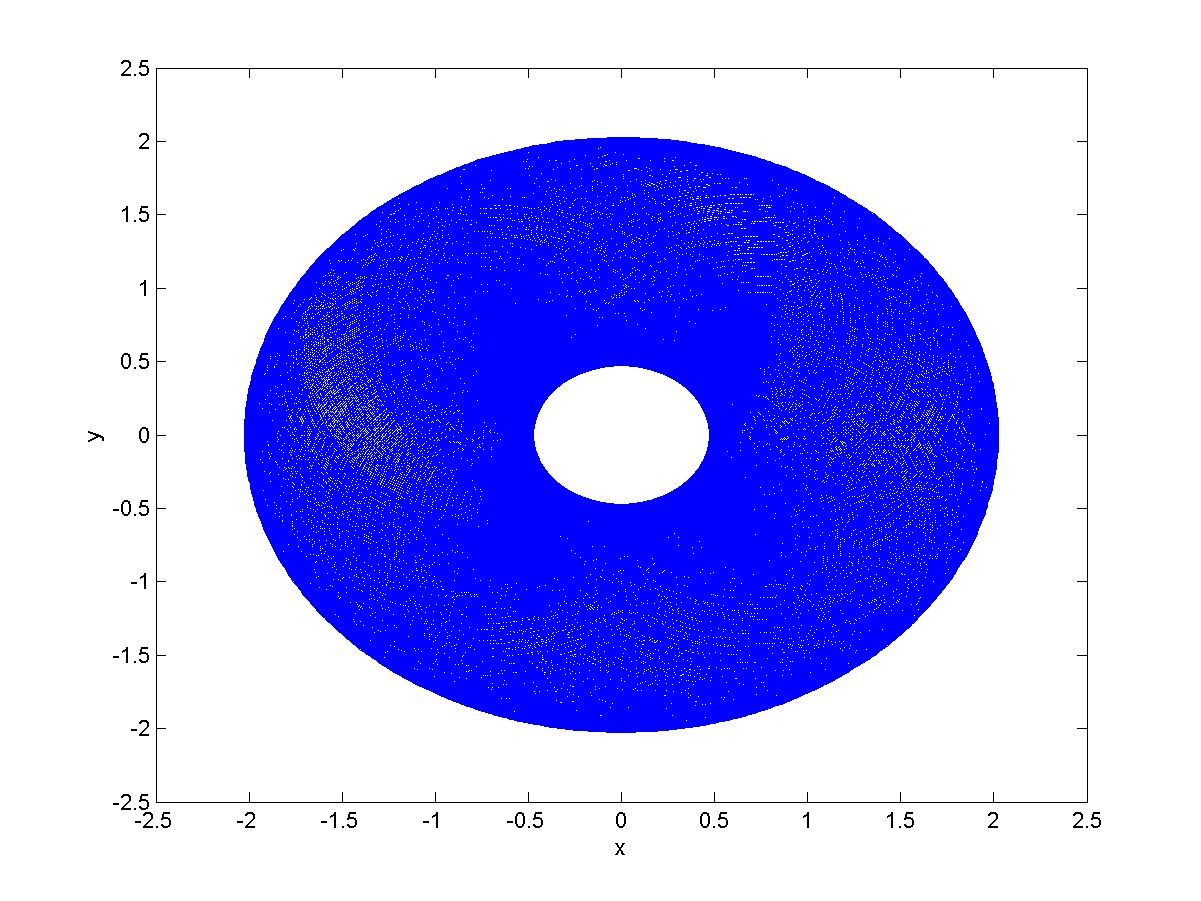
\includegraphics[width=\textwidth]{images/Q1_symplectique1_p.png}
    \caption{$p$ pour symplectique1}
    \label{fig:q1_symplectique1_p}
  \end{subfigure}
  ~
  \begin{subfigure}[b]{0.3\textwidth}
    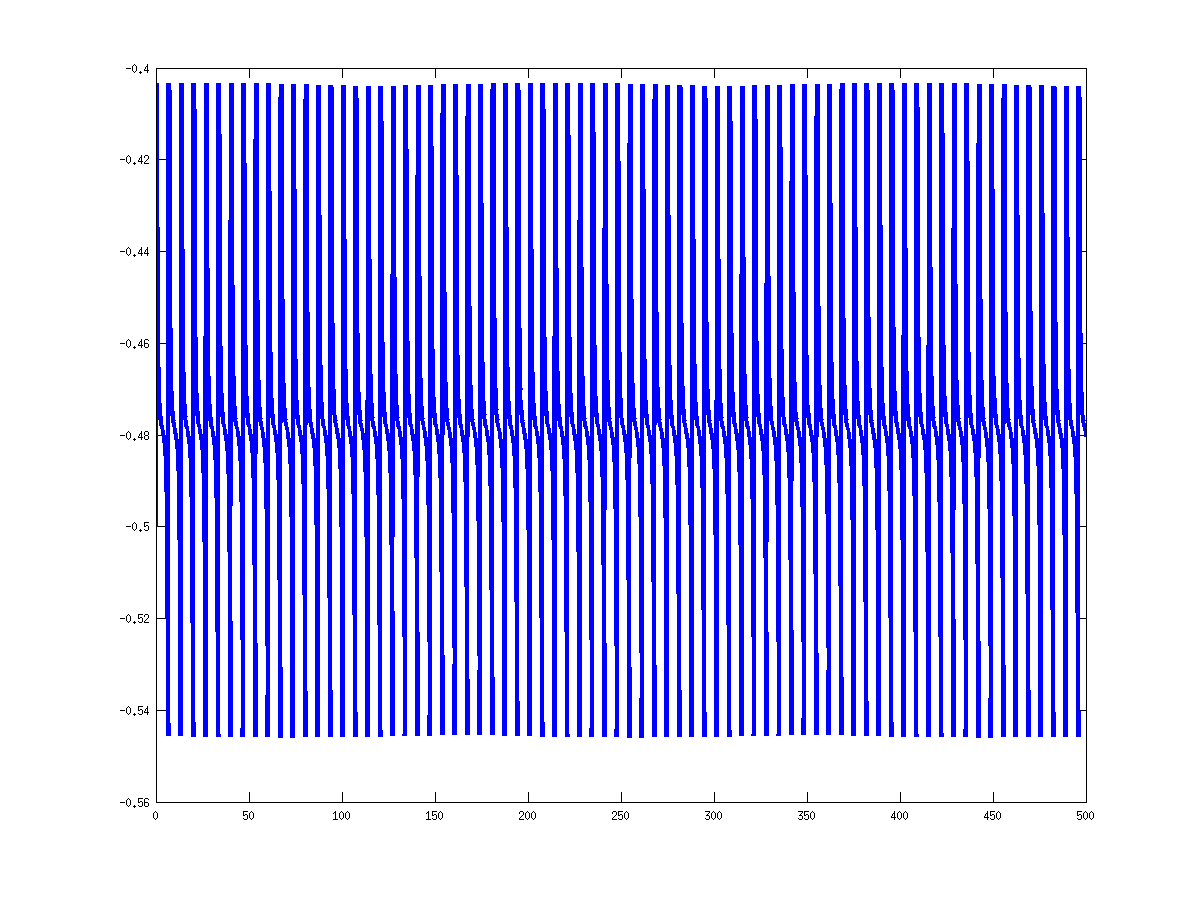
\includegraphics[width=\textwidth]{images/Q1_symplectique1_H.png}
    \caption{$\Ha$ pour symplectique1}
    \label{fig:q1_symplectique1_H}
  \end{subfigure}

  \begin{subfigure}[b]{0.3\textwidth}
    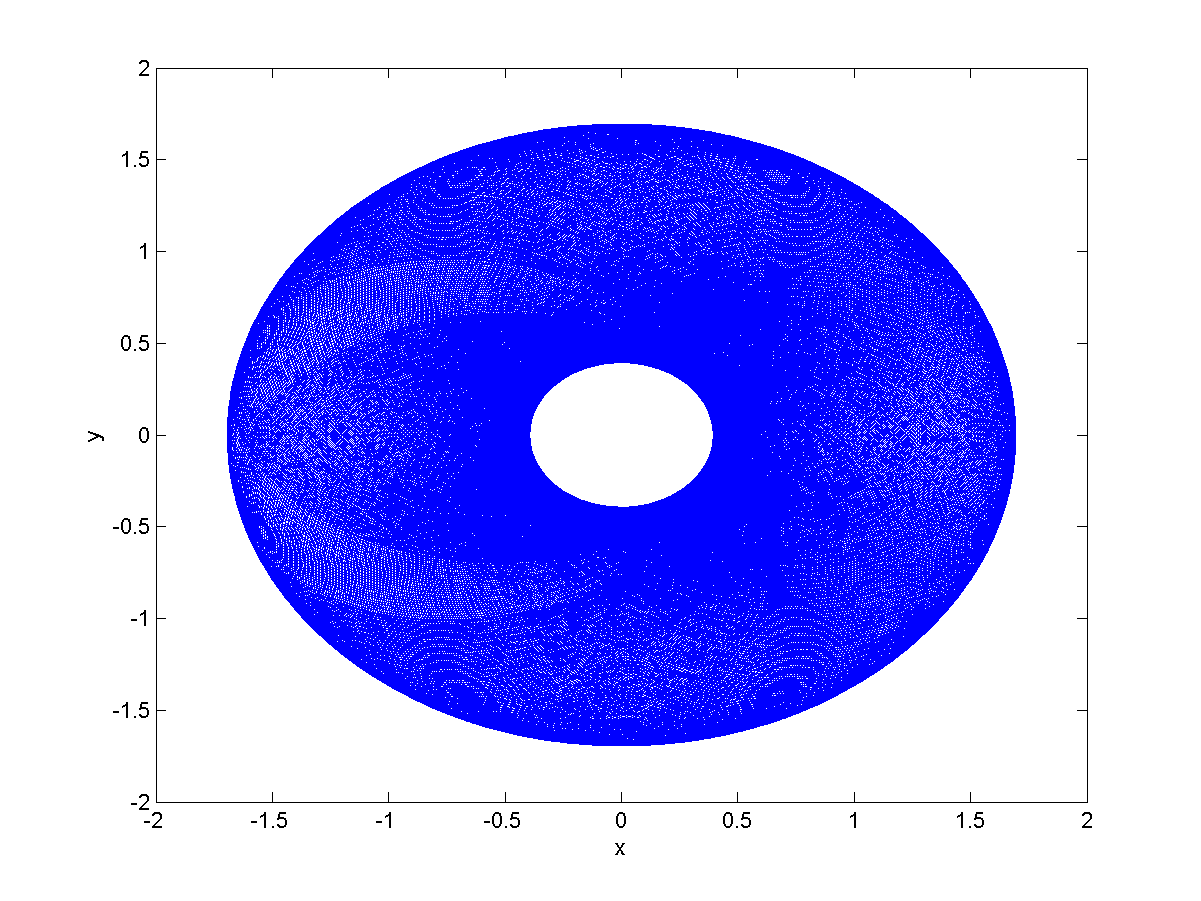
\includegraphics[width=\textwidth]{images/Q1_symplectique2_q.png}
    \caption{$q$ pour symplectique2}
    \label{fig:q1_symplectique2_q}
  \end{subfigure}%
  ~
  %(or a blank line to force the subfigure onto a new line)
  \begin{subfigure}[b]{0.3\textwidth}
    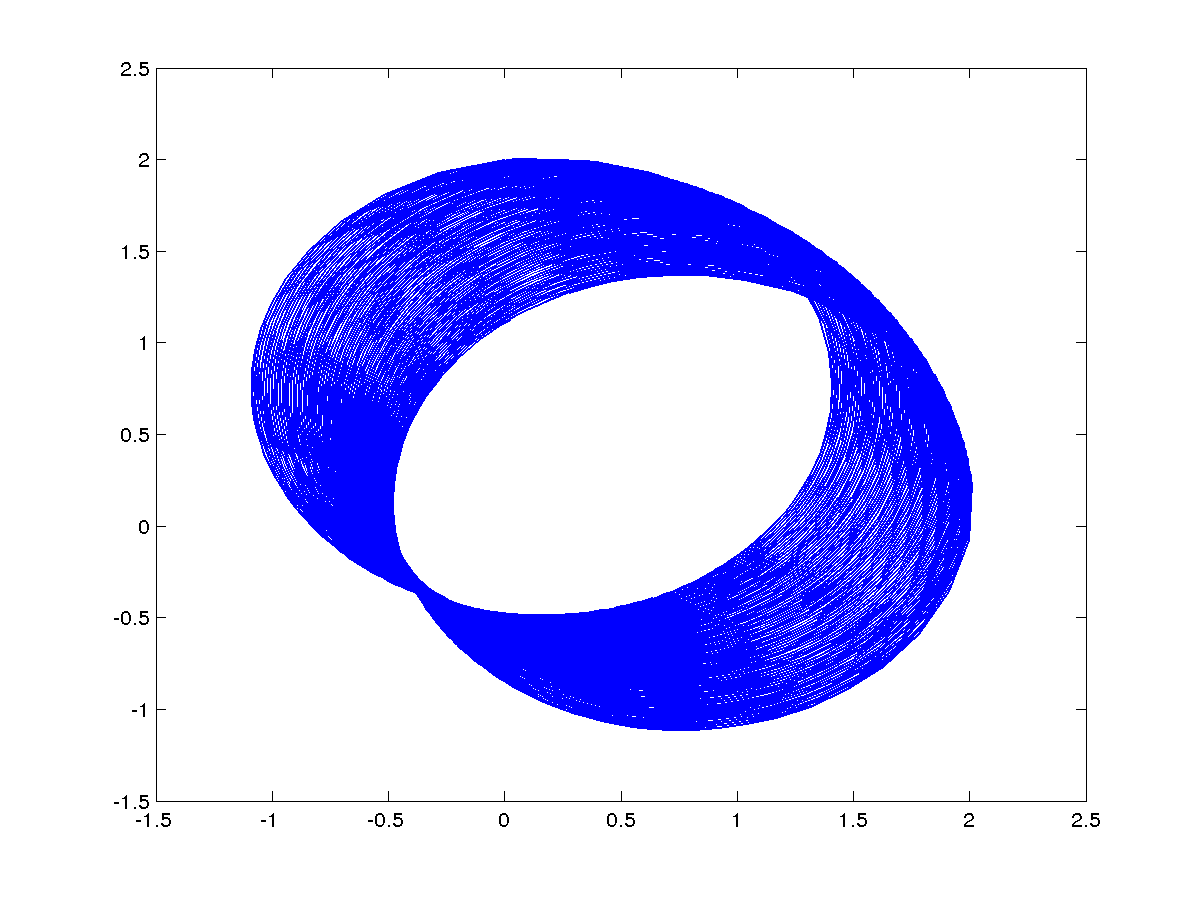
\includegraphics[width=\textwidth]{images/Q1_symplectique2_p.png}
    \caption{$p$ pour symplectique2}
    \label{fig:q1_symplectique2_p}
  \end{subfigure}
  ~
  \begin{subfigure}[b]{0.3\textwidth}
    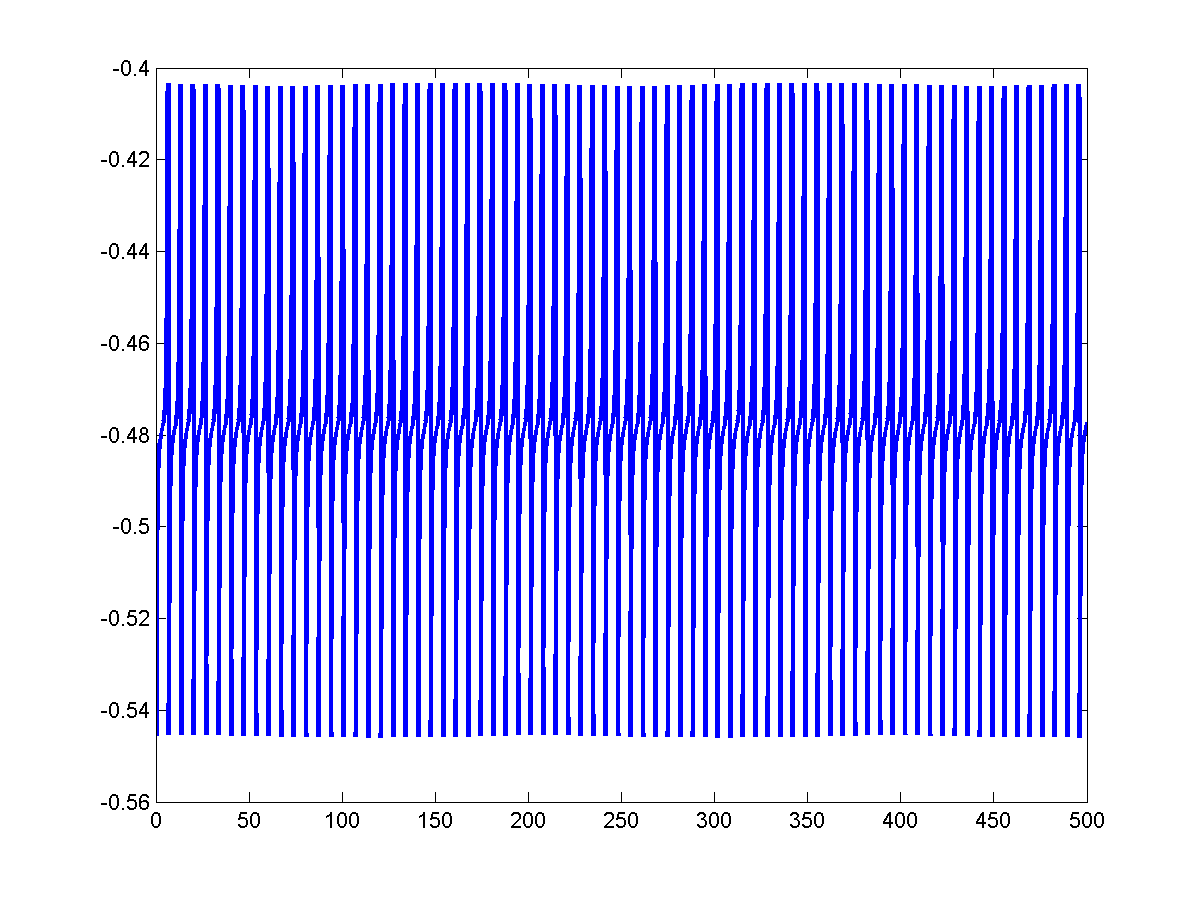
\includegraphics[width=\textwidth]{images/Q1_symplectique2_H.png}
    \caption{$\Ha$ pour symplectique2}
    \label{fig:q1_symplectique2_H}
  \end{subfigure}
  \caption{Résultats pour la question 1}
  \label{fig:q1}
\end{figure}


Les principaux points de comparaison des méthodes sont la convergence, l'erreur et le temps de calcul de la méthode.
















\section*{Question 2}
\subsection{Équations du mouvement}
Intéressons nous maintenant au cas où les deux corps sont de masse similaire. L'Hamiltonien du système doit bien entendu être redéfini, il est maintenant donné par 

$$\Ha(p_1,p_2,q_1,q_2) = \frac{1}{2} (\frac{1}{m_1} p_1^T p_1 + \frac{1}{m_2} p_2^T p_2) - G \frac{m_1 m_2}{||q_1- q_2||_2} $$

où $G$ représente la constante gravitationnelle et $m_i$ ma masse du corps $i$. On garde les mêmes conventions qu'à la question 1, c'est à dire que 
 $$q =
\begin{pmatrix}
  q_1\\
  q_2
\end{pmatrix},$$

$$p =
\begin{pmatrix}
  p_1\\
  p_2
\end{pmatrix},$$

avec $p_1$, $p_2$, $q_1$ et $q_2$ qui sont de la forme 
$$q_1 =
\begin{pmatrix}
  q_{11}\\
  q_{12}
\end{pmatrix},
q_2 =
\begin{pmatrix}
  q_{21}\\
  q_{22}
\end{pmatrix}$$
$$p_1 =
\begin{pmatrix}
  p_{11}\\
  p_{12}
\end{pmatrix},
p_2 =
\begin{pmatrix}
  p_{21}\\
  p_{22}
\end{pmatrix}
$$
 et
$f_1(q,p)$ et $f_2(q,p)$ sont tels que
\begin{align*}
  \dot{q} & = f_1(p,q)\\
  \dot{p} & = f_2(p,q).
\end{align*}

On calcule, en se rappelant des résultats de la question 1 mais en n'oubliant cependant pas d'inclure les masses, 
 
\begin{align*}
 f_{1,i}(q,p) &= m_i \fpart{\Ha(p,q)}{p_i} \\	
  f_1(p) & =
  \begin{pmatrix}
    m_1\frac{p_1}{m_1}\\
    m_2\frac{p_2}{m_2}
  \end{pmatrix}\\
  & = p\\
%	
 f_{2,i}(q,p) &= -\frac{1}{m_i}\fpart{\Ha(p,q)}{q_i} \\
  f_2(q) & = Gm_1m_2
  \begin{pmatrix}
    \frac{-(q_1-q_2)}{m_1\|q_1-q_2\|_2^3}\\
    \frac{(q_1-q_2)}{m_2\|q_1-q_2\|_2^3}
  \end{pmatrix}\\
  & = G
  \begin{pmatrix}
    \frac{-m_2 (q_1-q_2)}{\|q_1-q_2\|_2^3}\\
    \frac{m_1 (q_1-q_2)}{\|q_1-q_2\|_2^3}
  \end{pmatrix}.
\end{align*}

On obtient finalement notre système de 8 équations différentielles à 8 variables, qu'on va résoudre numériquement, comme dans la question 1, aux moyens des méthodes d'Euler explicite et symplectiques.\\
On choisit comme condition initiales : 
$$
q_1 = \begin{pmatrix}
0.4\\
0
\end{pmatrix},
q_2 = \begin{pmatrix}
0\\
0
\end{pmatrix},
p_1 = \begin{pmatrix}
0\\
2
\end{pmatrix},
p_2 = \begin{pmatrix}
0\\
-2
\end{pmatrix},
$$

\subsection{Analyse de la solution}

Commençons par calculer la jacobienne du système. Pour cela, calculons $\fpart{f_2}{q}$ :
$$
\begin{pmatrix}
\frac{Gm_2(2(q_{11}-q_{21})^2 - (q_{12} - q_{22})^2)}{||q||^5_2} & \frac{3Gm_2(q_{11}-q_{21})(q_{12} - q_{22}))}{||q||^5_2} & \frac{Gm_2(-2(q_{11}-q_{21})^2 + (q_{12} - q_{22})^2)}{||q||^5_2} & \frac{3Gm_2(q_{11}-q_{21})(q_{12} - q_{22}))}{||q||^5_2} \\
\frac{3Gm_2(q_{11}-q_{21})(q_{12} - q_{22}))}{||q||^5_2} & \frac{Gm_2(2(q_{12}-q_{21})^2 - (q_{11} - q_{21})^2)}{||q||^5_2} & \frac{3Gm_2(q_{11}-q_{21})(q_{12} - q_{22}))}{||q||^5_2} & \frac{Gm_2(-2(q_{12}-q_{22})^2 + (q_{11} - q_{21})^2)}{||q||^5_2} \\
\frac{-Gm_1(2(q_{11}-q_{21})^2 - (q_{12} - q_{22})^2)}{||q||^5_2} & \frac{-3Gm_1(q_{11}-q_{21})(q_{12} - q_{22}))}{||q||^5_2} & \frac{-Gm_1(-2(q_{11}-q_{21})^2 + (q_{12} - q_{22})^2)}{||q||^5_2} & \frac{-3Gm_1(q_{11}-q_{21})(q_{12} - q_{22}))}{||q||^5_2} \\
\frac{-3Gm_1(q_{11}-q_{21})(q_{12} - q_{22}))}{||q||^5_2} & \frac{-Gm_1(2(q_{12}-q_{21})^2 - (q_{11} - q_{21})^2)}{||q||^5_2} & \frac{-3Gm_1(q_{11}-q_{21})(q_{12} - q_{22}))}{||q||^5_2} & \frac{-Gm_1(-2(q_{12}-q_{22})^2 + (q_{11} - q_{21})^2)}{||q||^5_2} \\
\end{pmatrix}
$$

La jacobienne est donnée par : 
\begin{equation}
J(q,p) = 
\begin{pmatrix}
0 & I\\
\fpart{f_2}{q} & 0
\end{pmatrix}.
\end{equation}
Si on évalue $J(q,p)$ aux conditions initiales et qu'on calcul ses valeurs propres, on obtient : 
$$
\begin{pmatrix}
20.0431    \\
-20.0431   \\
-0.0000 +14.1726i \\
-0.0000 -14.1726i  \\
-0.0000          \\
-0.0000          \\
0.0000          \\
0.0000 
\end{pmatrix}
$$
On en conclut que le système n'est pas stable.\\

Intéressons nous maintenant aux résultats obtenus. 

	Comme l'illustre le graphe \ref{fig:q2_explicite_q}, dans le cas de la méthode d'euler explicite, les trajectoires tendent à s'éloigner au fil du temps. Ce qui est assez cohérent avec le graphe de la vitesse \ref{fig:q2_explicite_p}. En effet, sur ce dernier on constate que la vitesse augmente peu à peu, on saute de solution en solution, et donc forcément les corps peuvent parcourir une plus grande distance dans le même intervalle de temps, ce qui explique le graphe \ref{fig:q2_explicite_q}. L'énergie quant à elle augmente légèrement de manière globale  passant de $-2$ à $-1 \cdot 10^{-5}$ , mais par contre localement elle chute jusqu'à des $-7 \cdot 10{-5}$. 
	
	Ensuite pour Euler symplectique, on constate que les deux types renvoient les mêmes graphes tant pour p (\ref{fig:q2_symplectique1_p}, \ref{fig:q2_symplectique2_p}) que pour q (\ref{fig:q2_symplectique1_q}, \ref{fig:q2_symplectique2_q})  et $\Ha$ (\ref{fig:q2_symplectique1_H}, \ref{fig:q2_symplectique2_H}). Ce résultat, qui peut sembler surprenant de prime abord, est en fait cohérent. En effet, si on regarde de plus près on constate que dans les graphes de vitesse, cette dernière reste la même "à chaque tour", c'est à dire qu'on n'a pas d'erreur qui nous entraine vers une autre solution. Il en va de même pour la position qui, même si elle "monte" peu à peu à cause de l'interaction des deux corps, n'est en soit que la répétion d'un même mouvement. On n'a donc pas de risque de s'en aller vers l'une ou l'autre solution en fonction des variables sur lesquelles on applique euler explicite ou implicite.    



\begin{figure}
  \centering
  \begin{subfigure}[b]{0.3\textwidth}
    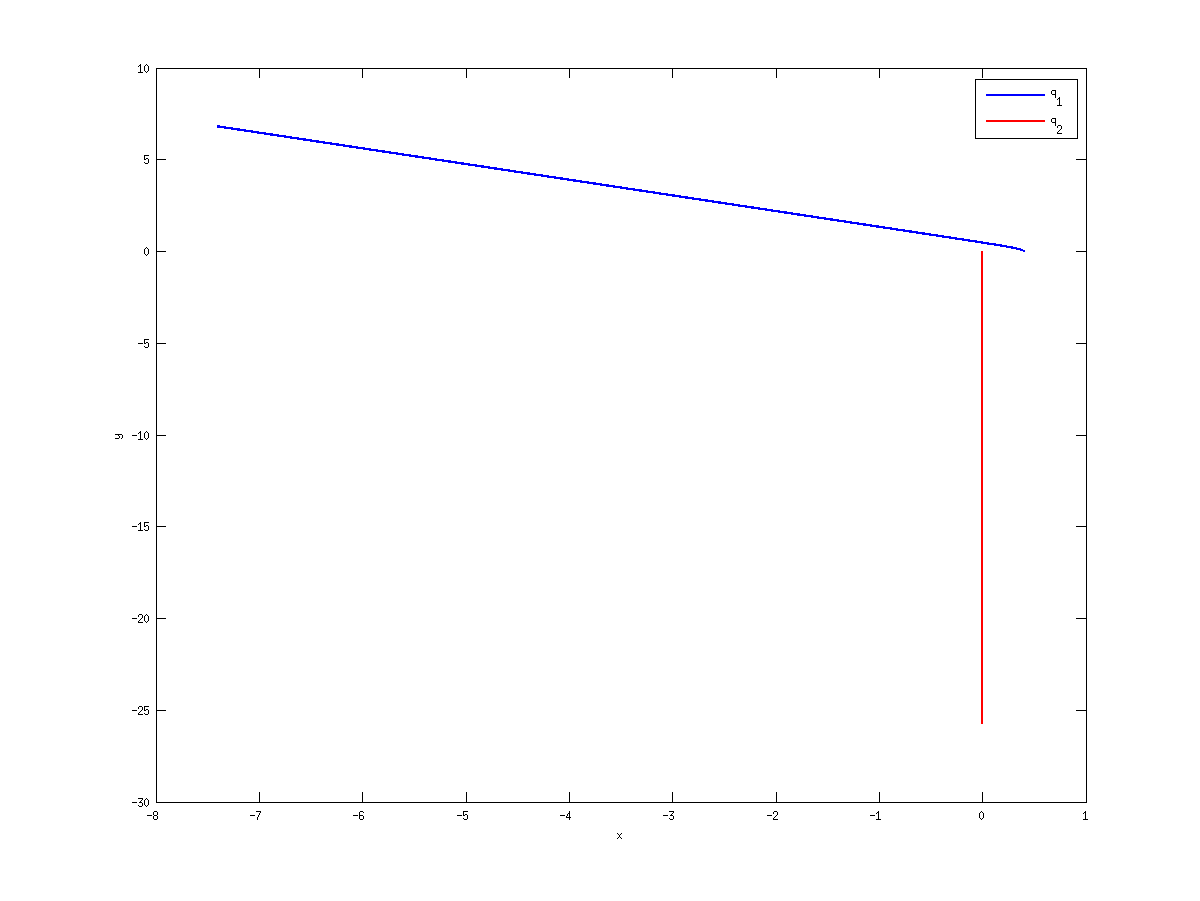
\includegraphics[width=\textwidth]{images/Q2_explicite_q.png}
    \caption{$q$ pour explicite}
    \label{fig:q2_explicite_q}
  \end{subfigure}%
  ~ %add desired spacing between images, e. g. ~, \quad, \qquad etc.
  %(or a blank line to force the subfigure onto a new line)
  \begin{subfigure}[b]{0.3\textwidth}
    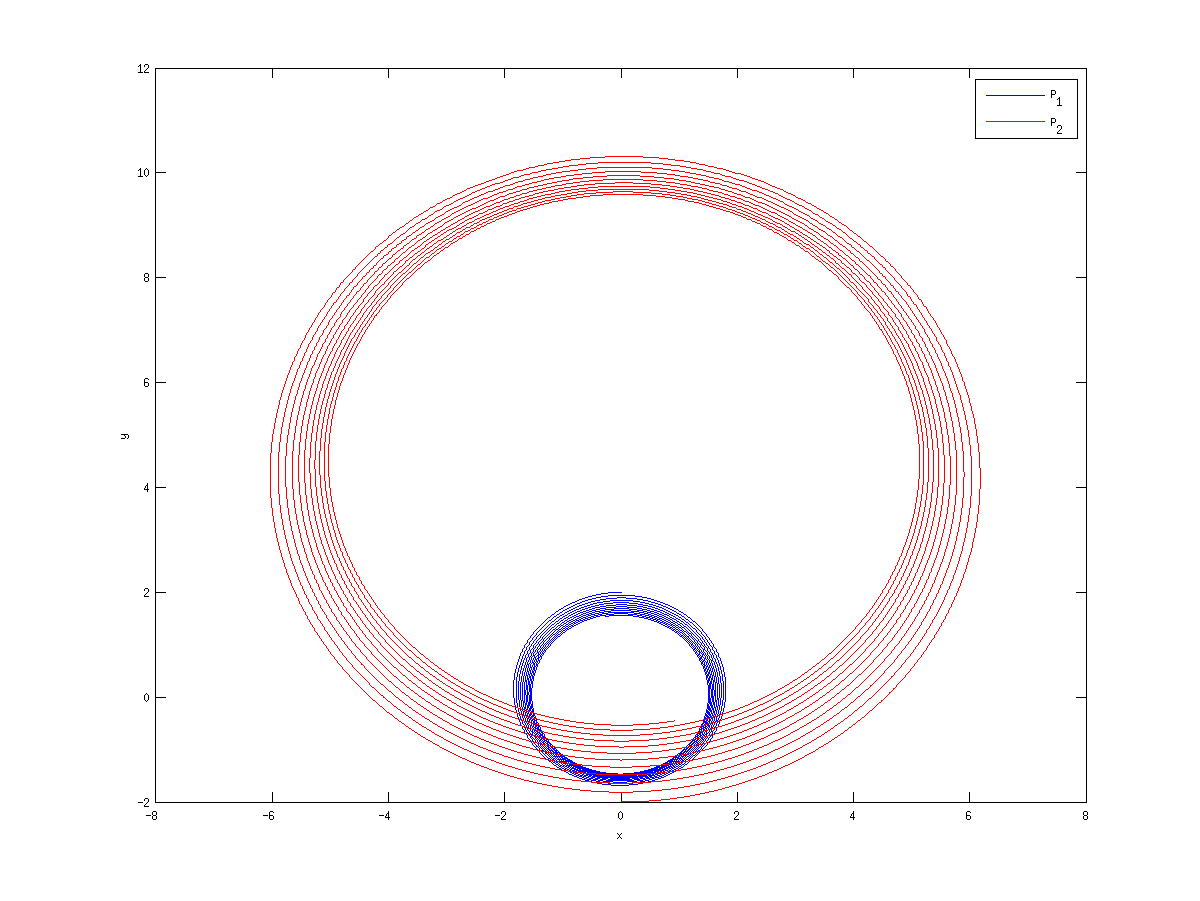
\includegraphics[width=\textwidth]{images/Q2_explicite_p.png}
    \caption{$p$ pour explicite}
    \label{fig:q2_explicite_p}
  \end{subfigure}
  ~
  \begin{subfigure}[b]{0.3\textwidth}
    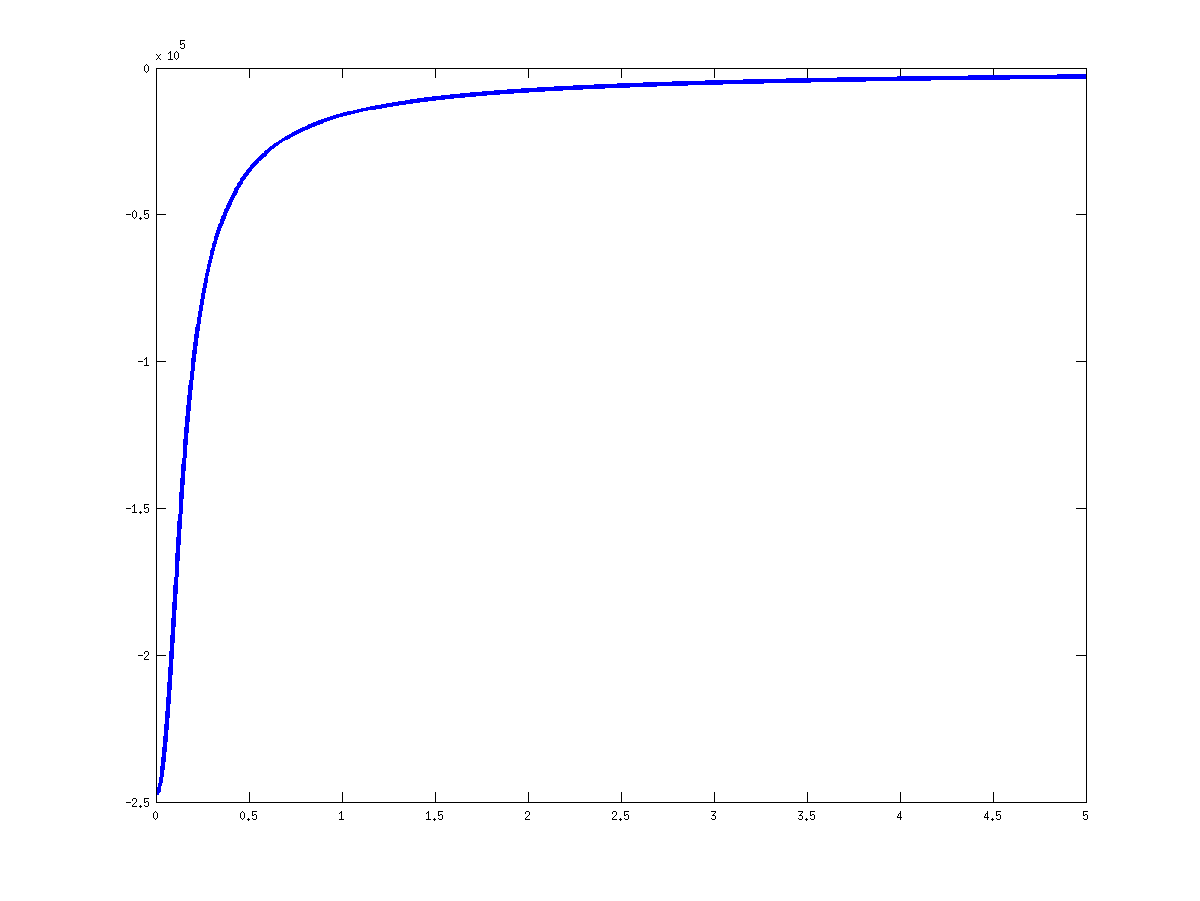
\includegraphics[width=\textwidth]{images/Q2_explicite_H.png}
    \caption{$\Ha$ pour explicite}
    \label{fig:q2_explicite_H}
  \end{subfigure}

  \begin{subfigure}[b]{0.3\textwidth}
    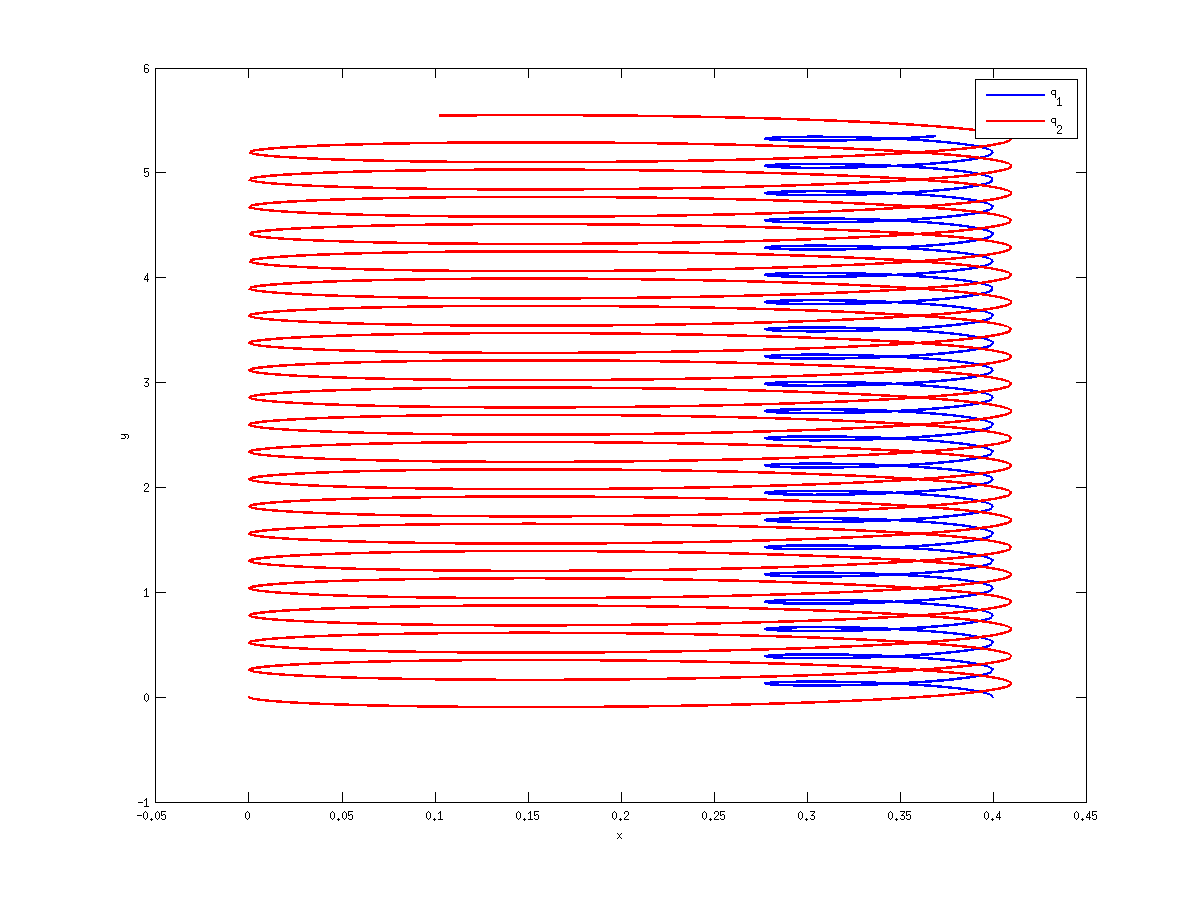
\includegraphics[width=\textwidth]{images/Q2_symplectique1_q.png}
    \caption{$q$ pour symplectique1}
    \label{fig:q2_symplectique1_q}
  \end{subfigure}%
  ~
  %(or a blank line to force the subfigure onto a new line)
  \begin{subfigure}[b]{0.3\textwidth}
    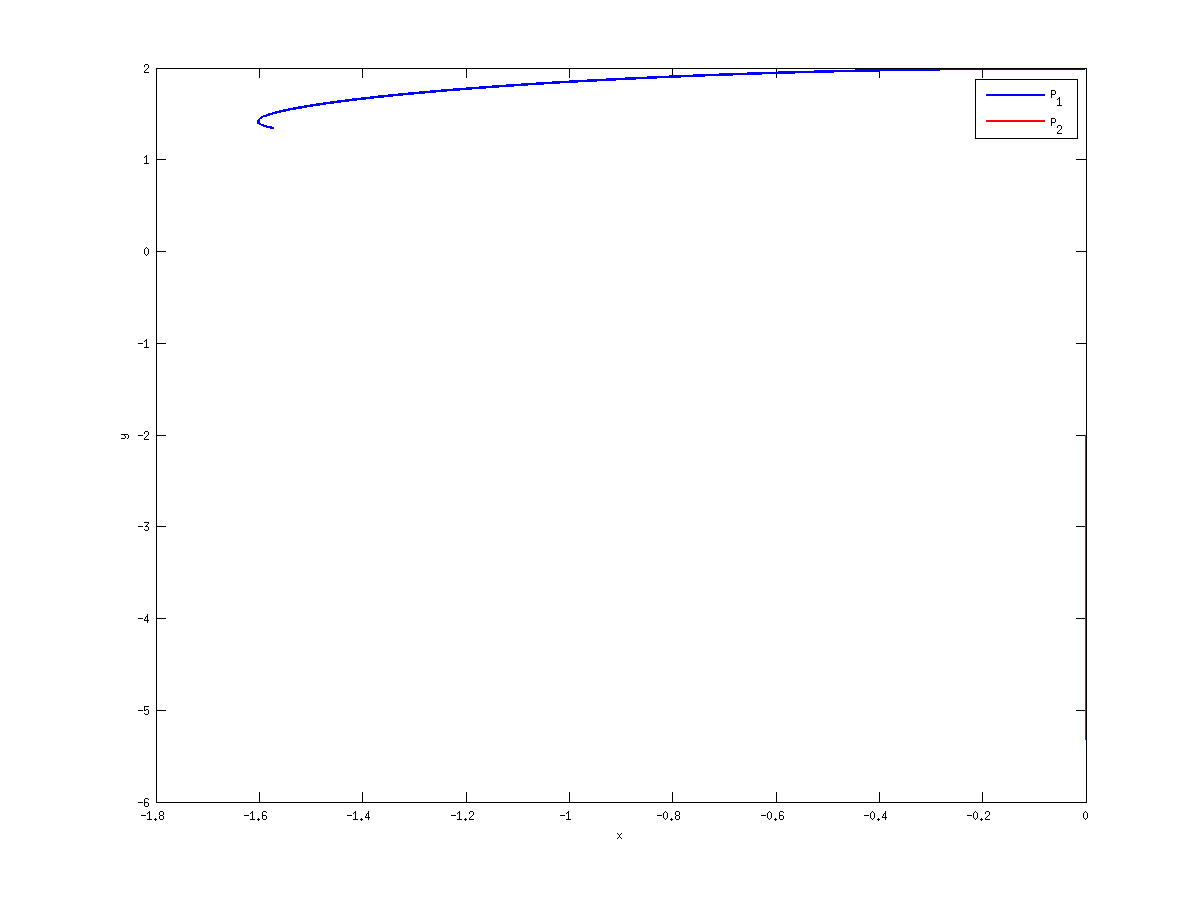
\includegraphics[width=\textwidth]{images/Q2_symplectique1_p.png}
    \caption{$p$ pour symplectique1}
    \label{fig:q2_symplectique1_p}
  \end{subfigure}
  ~
  \begin{subfigure}[b]{0.3\textwidth}
    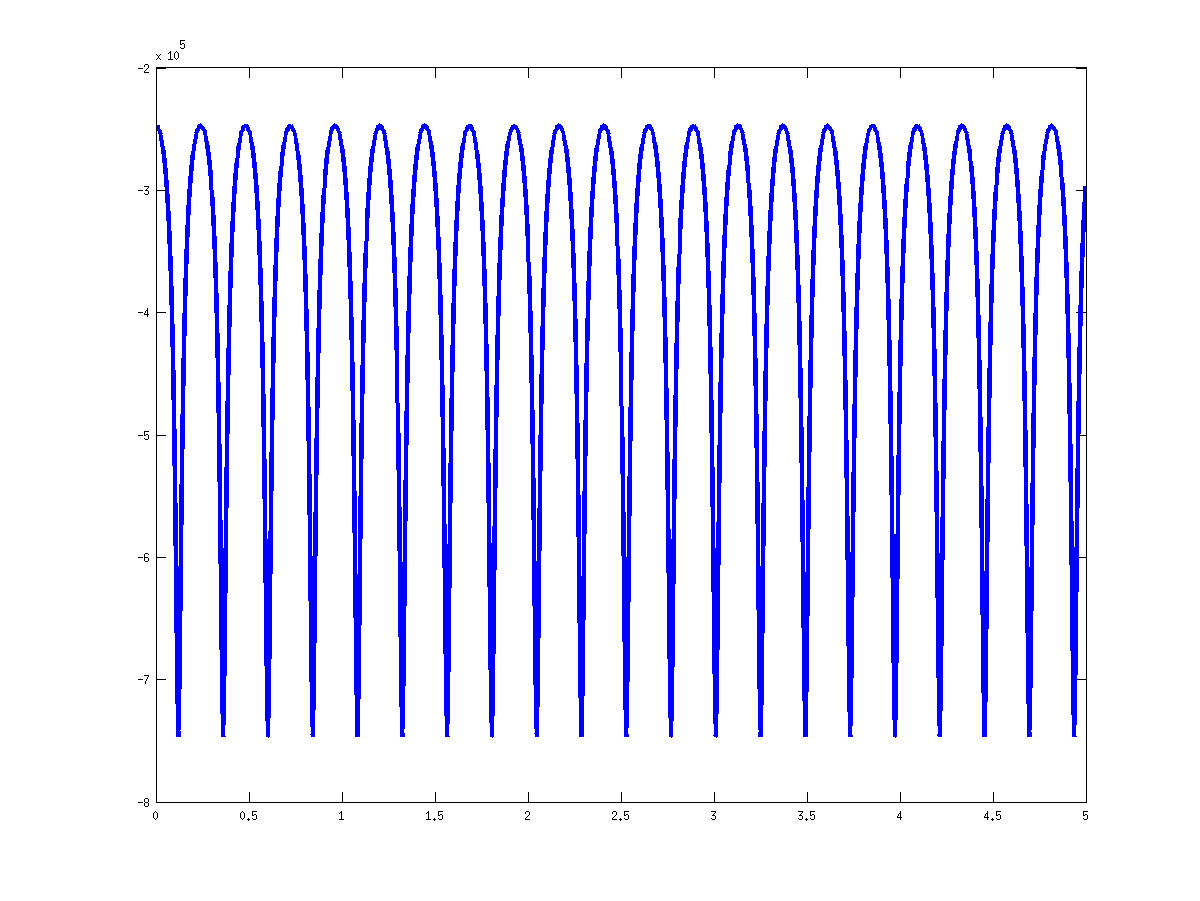
\includegraphics[width=\textwidth]{images/Q2_symplectique1_H.png}
    \caption{$\Ha$ pour symplectique1}
    \label{fig:q2_symplectique1_H}
  \end{subfigure}

  \begin{subfigure}[b]{0.3\textwidth}
    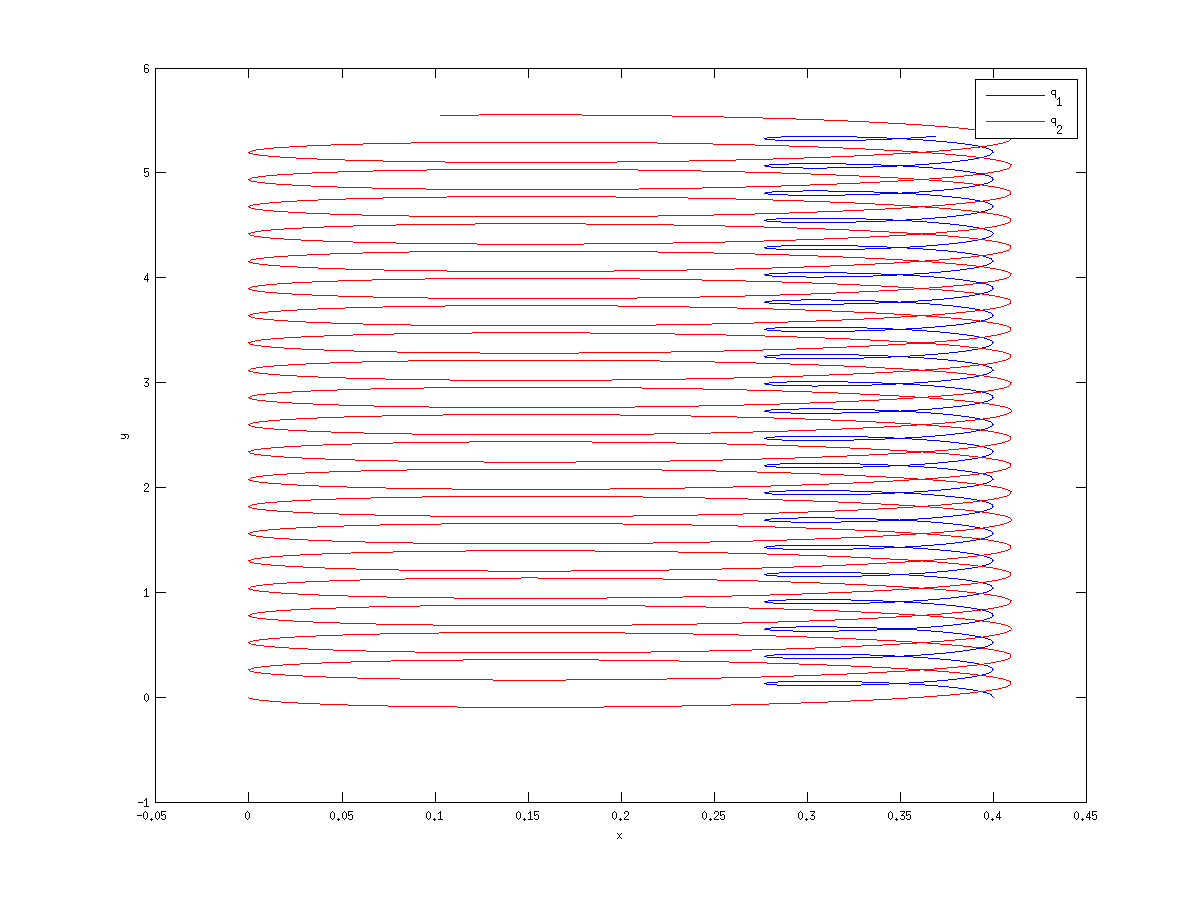
\includegraphics[width=\textwidth]{images/Q2_symplectique2_q.png}
    \caption{$q$ pour symplectique2}
    \label{fig:q2_symplectique2_q}
  \end{subfigure}%
  ~
  %(or a blank line to force the subfigure onto a new line)
  \begin{subfigure}[b]{0.3\textwidth}
    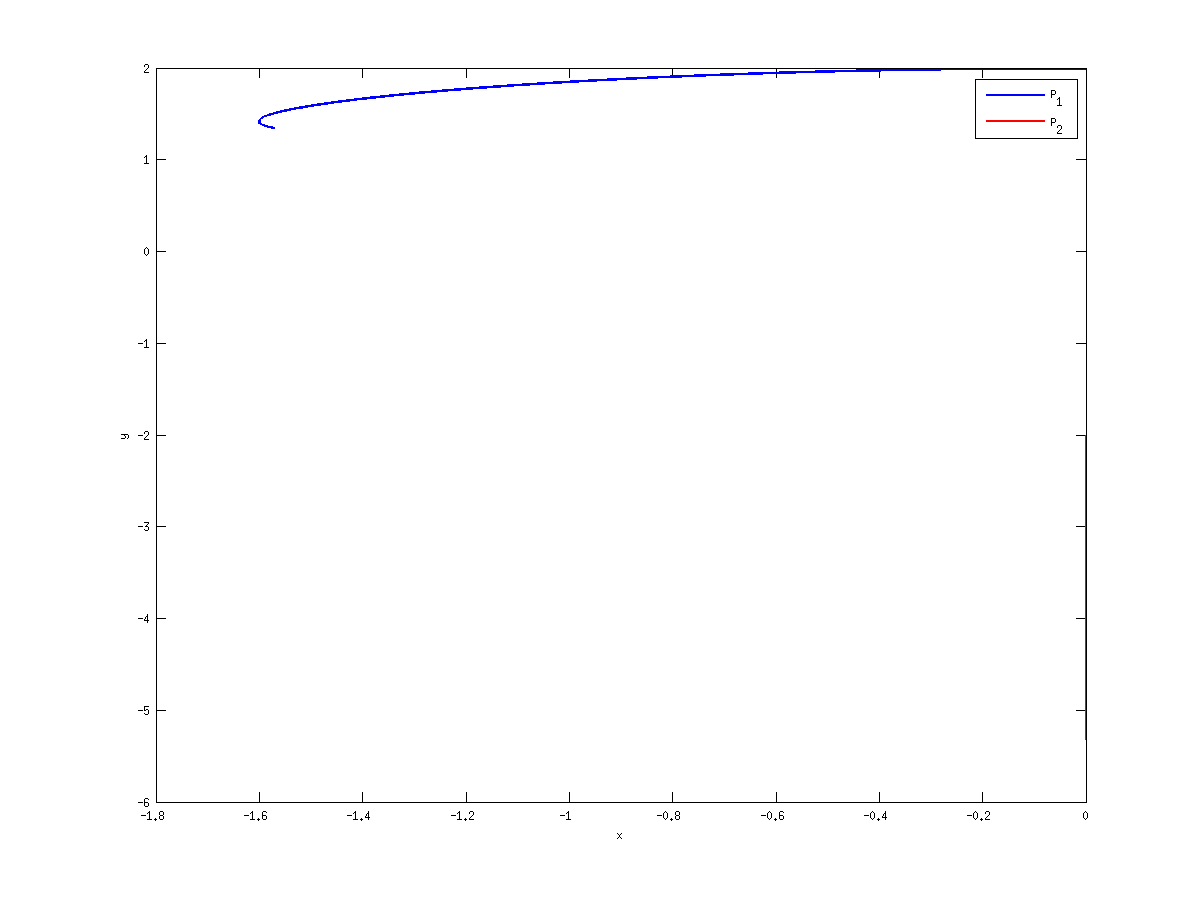
\includegraphics[width=\textwidth]{images/Q2_symplectique2_p.png}
    \caption{$p$ pour symplectique2}
    \label{fig:q2_symplectique2_p}
  \end{subfigure}
  ~
  \begin{subfigure}[b]{0.3\textwidth}
    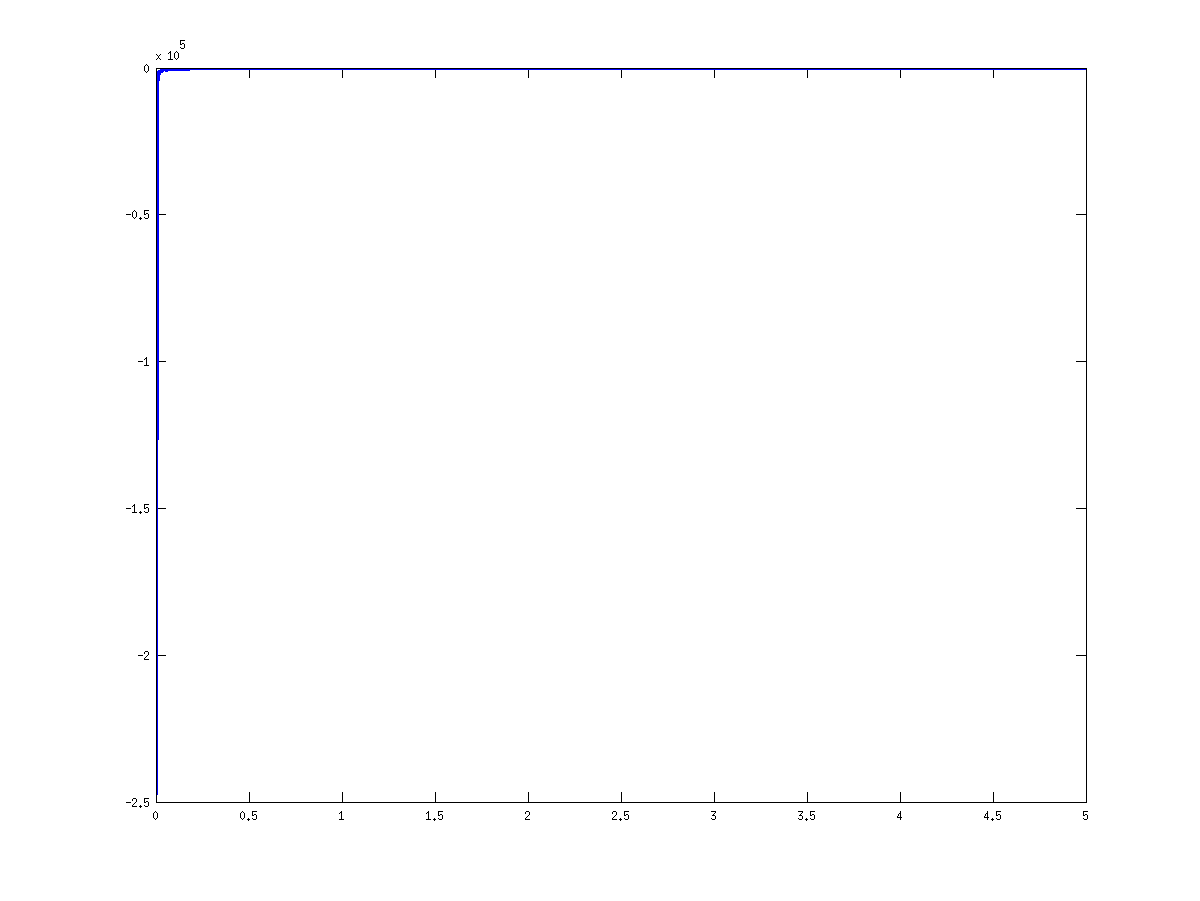
\includegraphics[width=\textwidth]{images/Q2_symplectique2_H.png}
    \caption{$\Ha$ pour symplectique2}
    \label{fig:q2_symplectique2_H}
  \end{subfigure}
  \caption{Résultats pour la question 2}\label{fig:q2}
\end{figure}


\end{document}
